\documentclass{standalone}
\usepackage{pgfplots}
\pgfplotsset{compat=1.18}
\usepgfplotslibrary{colorbrewer}
\pgfplotsset{cycle list/Set1-6}

\begin{document}

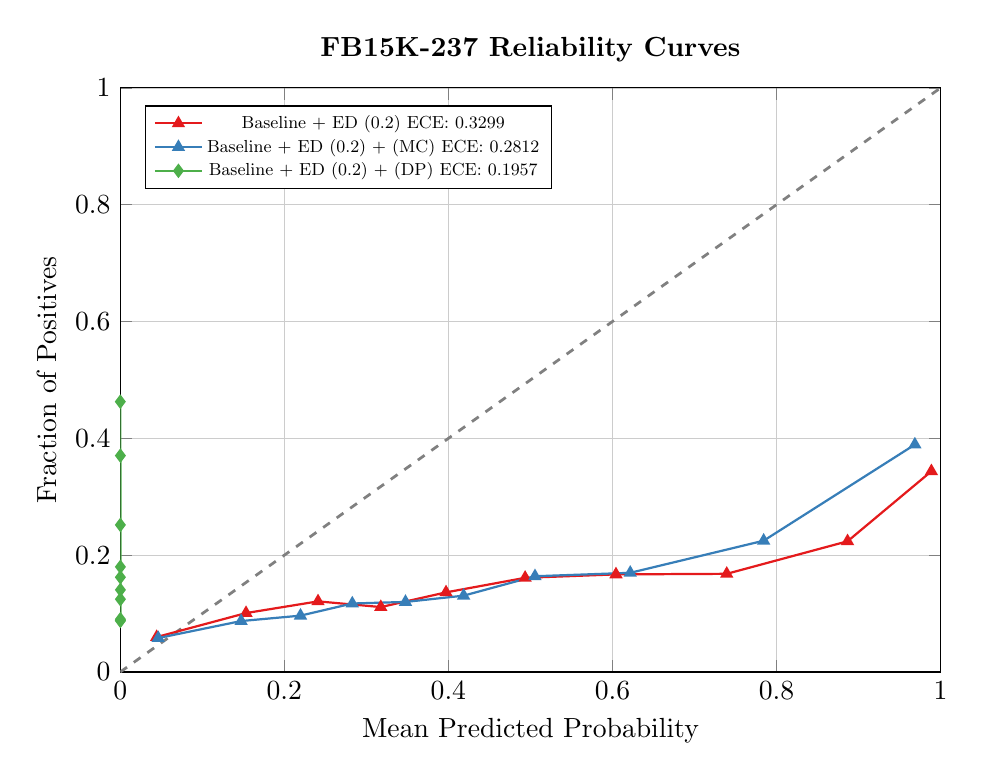
\begin{tikzpicture}
\begin{axis}[
    title={\textbf{FB15K-237 Reliability Curves}},
    xlabel={Mean Predicted Probability},
    ylabel={Fraction of Positives},
    xmin=0, xmax=1,
    ymin=0, ymax=1,
    xtick={0, 0.2, 0.4, 0.6, 0.8, 1.0},
    ytick={0, 0.2, 0.4, 0.6, 0.8, 1.0},
    legend pos=north west,
    legend style={nodes={scale=0.7, transform shape}, font=\small},
    grid=both,
    grid style={line width=.1pt, draw=gray!20},
    major grid style={line width=.2pt, draw=gray!40},
    width=12cm,
    height=9cm,
    cycle list name=Set1-6
]

% Perfectly Calibrated Line
\addplot [color=gray, dashed, line width=1pt, forget plot]
    coordinates {(0,0)(1,1)};

\addplot+[mark=triangle*, thick] coordinates {
    (0.04440314, 0.05984367) (0.15332946, 0.10090398) (0.24107407, 0.12093819) (0.31759084, 0.1111654) 
    (0.3970972, 0.13633032) (0.49352611, 0.16125092) (0.60428052, 0.16711459) (0.7393058, 0.16809186) 
    (0.8865653, 0.22379673) (0.98876647, 0.34367367)
};
\addlegendentry{Baseline + ED (0.2) ECE: 0.3299}

\addplot+[mark=triangle*, thick] coordinates {
    (0.04625737, 0.05813385) (0.14731774, 0.08722209) (0.21971495, 0.09650623) (0.28285926, 0.11727339)
    (0.34768092, 0.11996091) (0.41855987, 0.13071097) (0.50555681, 0.16393843) (0.62166645, 0.1698021)
    (0.78429812, 0.224774) (0.9686335, 0.38935027)
};
\addlegendentry{Baseline + ED (0.2) + (MC) ECE: 0.2812}

\addplot+[mark=diamond*, thick] coordinates {
    (8.85968281e-05, 0.46278871) (1.43167269e-04, 0.25178215) (1.73005878e-04, 0.16224693) (1.82264527e-04, 0.09039065)
    (1.84048393e-04, 0.08836944) (1.85055201e-04, 0.08756418) (1.85721162e-04, 0.12460793) (1.86234902e-04, 0.17992586)
    (1.86682950e-04, 0.37040205) (1.89608481e-04, 0.14057599)
};
\addlegendentry{Baseline + ED (0.2) + (DP) ECE: 0.1957}


\end{axis}
\end{tikzpicture}

\end{document}